\chapitre{Trio pour clarinette, violon et … trombone, le 18 juillet 2033}{Les sabots de frein geignant,}{ Timothée se stationne comme il le fait du lundi au vendredi, à la même heure, devant sa maison, une imitation de cottage anglais particulièrement mal réussie. Pourquoi endure-t-il le revêtement de bardeaux d’amiante blancs remontant au siècle dernier ? Ne sont-ils pas cancérigènes ? Pourquoi ne les fait-il pas recouvrir de planches synthétiques ? Il ne le fait pas parce qu’il n’a pas de sous. Il a deux parents, sans oublier leur sale bête de chien-rat, à nourrir, à vêtir, à soigner, à soutenir, à rassurer, à protéger. À cacher !}

Un chatouillement lui titille l’oreille.

- Timothée Tardif !

- Monsieur Tardif ? Allanah Desrosiers de la Caisse populaire de Rimouski, vous allez bien ?

- Euh …

- Je vous appelle parce que votre compte chèque est à découvert de 97,64 \$.

- Ah !

- Vous allez vous en occuper avant demain matin 9 h ?

- Euh …

- Parfait, Monsieur Tardif, au revoir !

L’homme s’escrime quelques instants avec sa portière aux gonds à moitié pourris, réussit à sortir de sa traction américaine et se retourne pour agripper deux sacs d’épicerie, deux «extra-forts jetables et 100 % compostables». Ce faisant, il réalise que Louis-Marc Richard est, encore une fois et comme toujours, en train de l’écornifler.

Du côté fleuve de la très fleurie rue Crouet, il n’y a qu’une maison, celle de Timothée, une construction artisanale de deux étages, sans parler de son prodigieux sous-sol, laquelle fut érigée en 1970 sur la crête de l’à-pic escarpement, avec triple ancrage bétonné sous la chaussée, ce qui nécessita certains accommodements à la Ville. C’était le seul endroit possible du versant nord; plus à gauche, le haut de la falaise est trop étroit et à droite, c’est le terrain du cimetière nazaréen qui débute. Rapidement, l’invraisemblable cottage se métamorphosa en curiosité qu’on vint voir. Du coup, le voisin d’en face perdit sa vue sur le Saint-Laurent, ses couchers de soleil sur la Côte-Nord et sa belle tranquillité.

Lorsqu’il prit sa retraite en 2010, il vendit son énorme bungalow à Louis-Marc Richard lequel, à son tour, commença à détester l’affligeante bicoque qui lui obstruait le panorama. Tellement, dit-on, que tous les jours, il fait une prière pour qu’elle s’écroule sur la voie ferrée au pied du cap et, qu’au même moment, un convoi ferroviaire la pousse sur les battures noirâtres du fleuve.

Quand, il y a dix ans, Richard apprit que l’inquiétante propriété avait changé de mains, il espéra, un instant, que l’acheteur l’améliorerait, l’embellirait, l’arrimerait davantage à l’esthétique ambiante de la rue et de sa dizaine de maisons. Mais non, rien ne se produisit, pas un coup de marteau ne fut entendu. Ses espoirs furent cependant ravivés cinq ans plus tard, en apercevant un fardier y livrer des feuilles de gypse, des panneaux de contreplaqué, du bois en formats variés, une immense fenêtre à espagnolette et tout le nécessaire pour effectuer des travaux majeurs. Mais encore là, ce fut une déception. Tout disparut à l’intérieur.

- Dis donc, voisin, lui avait-il demandé, tu rénoves ?

- Je construis un logement dans le sous-sol.

- Pour toi ?

- Non. Pour louer.

- À des locataires ?

- À des locataires.

- Mais y en a pas dans notre rue !

Timothée lui avait alors tourné le dos et s’en était retourné à ses occupations. Offusqué, furibond, Richard l’avait mortellement haï et, depuis, il ne lui avait plus jamais parlé. Dans un premier temps, il avait bien remarqué qu’une porte d’entrée avait été aménagée sur la façade permettant d’accéder directement au logement. Mais, quelques mois plus tard, elle avait été bouchée, laissant paraître cette affreuse cicatrice que l’on pouvait encore contempler aujourd’hui. Louis-Marc Richard supposait que son vis-à-vis avait changé d’idée pour les locataires – en fait, il n’en avait jamais vu l’ombre d’aucun – et qu’il avait tout simplement agrandi son espace vital. Oui, mais pourquoi ?

Cet étrange voisin qui ne recevait jamais de visite, qui semblait toujours seul et … sans femme, occupait déjà un grand rez-de-chaussée et, par surcroît, un étage assez spacieux pour abriter deux chambres normales. Pourquoi lui fallait-il un sous-sol en plus ? Lui, un célibataire dont la voiture était un outrage à la rue Crouet et la tenue vestimentaire, une illustration de misère noire. Sans parler de ce chien jaune qu’on avait envie de fesser à coups de pied, une bête sournoise qu’il se contentait d’envoyer marcher par GPS quand il y pensait. Étrange ! Bizarre ! À surveiller !

C’est ce qu’il fit, se mettant même à évaluer le volume des sacs d’épicerie que Timothée charriait parfois tous les jours en fin d’après-midi. Comment un homme seul d’apparence aussi modeste, pouvait-il manger autant que les trois Richard réunis, le père et ses deux ados ? Intrigant !

\begin{floatingfigure}[r]{60mm}
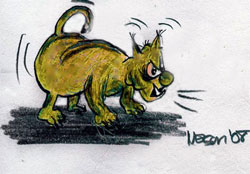
\includegraphics[height=35mm]{corps/chapitre4/img/gazou.jpg}
\end{floatingfigure}

Timothée hausse les épaules et, sacs en main, disparaît à l’intérieur. Sans s’arrêter dans sa tanière, il dévale directement un escalier à pic et tout en bas, cogne du pied. Mais déjà, Gazou l’a repéré et s’est mis à aboyer avec furie, son sale museau de fausset tout plissé par la haine. Heureusement, un ordre susceptible d’intimider un adjudant-chef d’infanterie se fait entendre :

- Ichi ! À côté de Maman !

Instantanément, le chien-rat se tait et Timothée franchit le seuil de la porte. L’un retourne s’écraser près du fauteuil de sa maîtresse, l’autre salue gauchement. Habitué aux senteurs ambiantes, il les ignore et va placer les provisions sur le comptoir de la cuisinette. En passant, il dépose les quatre livres de poche remis par l’ancienne bibliothécaire sur une pile de bouquins non classés.

- Au moins, ils ont sorti les vidanges, remarque-t-il.

À son père qui l’a suivi pour l’aider, il glisse un petit dix onces de vodka que le bonhomme a tôt fait de cacher dans une armoire. Puis, à voix basse

- L’écornifleux m’a encore guetté.

- Penses-tu qu’il commence à soupçonner quelque chose ?

La question reste sans réponse. Comment savoir ? S’il y a danger d’être dénoncé, ça ne peut venir que de Louis-Marc Richard. Les autres résidents de la rue sont trop éloignés pour remarquer quoi que ce soit, pour se douter de quelque chose. Et, en dix ans, mis à part Richard, personne ne lui a jamais adressé la parole, personne n’a jamais paru s’intéresser à lui, personne n’en a eu besoin.

- Merci pour tout ça, Timothée-Milet.

Quand son père l’appelle ainsi, c’est qu’il est heureux de sa présence et qu’il a envie d’échanger, de raconter, de rire.

- As-tu vu, vous recommencez à avoir des fourmis, fait le fils en écrapoutissant trois bestioles prises en flagrant délit d’écorniflage sur le comptoir.

Le vieillard se tord les maxillaires en un sinistre bâillement et s’en retourne s’écraser dans son fauteuil malgré la Maririou qui psalmodie son habituelle liturgie. Elle en a long à dire. Mais Timothée ne l’écoute pas lui non plus. Il garde plutôt les yeux fixés sur cette immense fenêtre pleine de lumière d’où il peut voir le fleuve évoluer autour des îles Canuel et Saint-Barnabé. En même temps, il pense à tous ces gens heureux qu’il a croisés en route. À ces filles qui riaient. À ces filles écourtichées et immodestes qui vivaient débordantes de santé, de jeunesse, d’insouciance. Finiront-elles comme Luce Morency ? Allez savoir ! Mais dans ce coq à l’âne onirique, le masque hargneux de Louis-Marc Richard, une figure fielleuse, toxique, mortelle, vient durement chasser celui triste et perdu de la démente. Et voilà qu’à son tour, il cède la place à celui du bonhomme Martel et à ses insinuations sur son Saguewanish, puis, swoosh !, aux traits tout en sourire, en simplicité et en politesse surannée de Bea Bellow.

Bea Bellow, les Giono ! Timothée a tôt fait de repérer les livres promis sur un des rayons à gauche de la fenêtre.

\begin{floatingfigure}[l]{40mm}
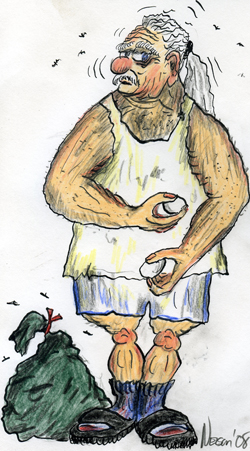
\includegraphics[height=60mm]{corps/chapitre4/img/romain1.jpg}
\end{floatingfigure}

Pendant ce temps, chattemite incorrigible, Romain augmente subrepticement le volume de son écouteur sans fil; l’heureux homme n’entend plus le flot récriminatoire de sa conjointe; savoir utiliser son expérience à bon escient constituerait, dit-on, une preuve d’intelligence. Timothée, lui, a droit au grand jeu. Il a mis trop de temps à revenir de son travail. Il a traîné. À quoi a-t-il pensé ? Voit-il une femme ? On espère bien que non ! A-t-il bu ? Eux autres, les vieux, ils commençaient à s’inquiéter ! Qui peut prévoir une descente de police ? Le BAG frappe toujours sans prévenir. Et patati et patata.

Puis voilà que soudain, sans qu’on ne le sente venir, elle se tait. Consciente de célébrer un cérémonial essentiel à sa vie, elle se saisit du violoncelle debout près de son fauteuil. C’est le signal ! Immédiatement, Gazou file se cacher sous un lit et les deux hommes, résignés, vont au placard chercher leur instrument, le fils un trombone, le père une clarinette.

- Trio pour clarinette, violonchelle et piano, opuch 2 de Vinchent d’Indy, chuinte la mère. Pis toi. Gajou, tu te tais, sinon tu vas avoir affaire à Maman !

Avec son trombone, instrument qu’il déteste de plus en plus et qu’il a cessé de maîtriser depuis belle lurette, à preuve les couacs intermittents, Timothée suit sans plaisir la partition bricolée par sa mère, faute d’avoir un piano. Mais il finit néanmoins par se rendre au bout. Avec son trombone, il ne peut évidemment rendre justice à l’opus original qui a été composé pour clarinette, violoncelle et piano. Il le sait. Et sa mère aussi. Sauf que cette contrariété lui donne une occasion supplémentaire pour se dire déçue de ce fils paresseux, un enfant qui avait tellement de talent musical, tellement de potentiel. Une nouvelle litanie est lancée et sur le point de passer au crescendo. Mais Romain en a assez; il s’immisce.

- Là, tu vas arrêter. Je te rappelle que Timothée, un «travaillant» du CRG où on garde les vieux comme nous autres en cage, nous cache ici, dans sa maison, et paie tout de sa poche. S’il se fait prendre, il est fini pour le reste de ses jours. Tu vas lui sacrer patience. Ça n’a pas de maudit bon sens !
Marie se tait. Elle regarde fixement son homme, puis, façon d’admettre qu’elle a eu tort, elle baisse la tête vers Gazou qui est revenu et qui gronde en direction du vieillard. Ignorant Timothée, elle se lève et marche, l’animal grotesque à sa suite, jusqu’à la cuisine. Peut-être qu’elle va y apercevoir quelques fourmis et se défouler sur les malheureux hyménoptères, se dit Timothée. Mais, au son, elle semble plutôt vouloir bardasser. Il lui faut ramasser la vaisselle du midi et préparer le repas du soir.

Avant, Romain ne rouspétait jamais. Il laissait toujours «border», ce qui convenait parfaitement bien au caractère invivable de la Maririou. Mais, avec les années, il lui a fallu réduire, raréfier, puis arrêter sa consommation de hash; la substance ne lui réussissant plus, le bien-être ayant été remplacé par la paranoïa et l’angoisse. Pire, il y avait eu l’été 2027 et cette affaire ratée depuis laquelle, tous deux étaient reclus. Voilà qui suffit amplement à changer un caractère.

Ému, le fils se lève à son tour, va ranger son instrument, caresse timidement l’épaule de son père en passant et, escorté par Gazou qui essaie vicieusement de lui mordre un mollet, s’engage dans l’escalier.

- Couché Gazou, méchant chien !

Et si jamais Robespierre Alcide lui fournissait les petites pilules du bonheur, ces cachets sans lendemain, qu’en ferait-il ? Comment aborderait-il la question avec son père, avec la Maririou ? «Tenez, avalez ça avec un verre d’eau. Ne craignez rien, ce n’est pas souffrant, c’est comme un somnifère, un gros gros somnifère ! Un somnifère pour toujours !» N’y a-t-il pas une autre solution ? Une façon différente de vivre ? Ça n’a plus de bon sens. L’agressivité, la vindicte, l’acrimonie semblent en escalade constante. Et leur aire d’habitation aux vieux, elle mériterait un grand ménage au savon fort, au plâtre, à la peinture, une rénovation importante avec des rideaux neufs, des meubles moins cabossés. Ça sent mauvais, c’est sale, humide, étouffant, déprimant.

Il est vrai que sa mère tire souvent de trop gros boulets sur de trop petites cibles, mais quand même. Il faut comprendre le contexte pénible dans laquelle elle vivote depuis six ans. C’est comme si on avait mis en cage une lionne de la savane, une lionne dans la force de l’âge avec le museau taché de sang. Pour une personne qui, comme elle, en menait large dans l’univers culturel de la région, la situation est carrément invivable. Et c’est ainsi depuis six ans !

Jeune fille volontaire, opiniâtre, studieuse, travailleuse, bûcheuse, non diplomate, incapable d’humour, toujours sérieuse et, généralement, insupportable, elle s’est retrouvée en 1972, elle avait 21 ans, Premier Prix du Conservatoire de musique de Québec en violoncelle. Ensuite, elle a joué comme remplaçante avec l’Orchestre symphonique de Québec, ainsi qu’avec la Société de musique contemporaine du Québec. De là, elle est passée en France où, avec son caractère éprouvant, elle a bourlingué un peu partout, mais surtout dans le Midi. Des gens ont pleuré à cause d’elle, aussi bien par amour que par haine.

Puis, à 29 ans, elle est revenue au pays lors d’une tournée avec l’Orchestre de Chambre de Toulouse. Forcée au repos, elle a alors découvert un projet d’école populaire de musique, un projet anarchique qui devint, au fil des ans, une institution régionale ayant ses hauts et ses bas et qu’elle appuiera jusqu’à la fin, en 2021. L’idée était noble: transférer des rudiments de musique aux moins bien nantis de la société. Évidemment son caractère n’aidant pas, elle y sema bisbille et zizanie, s’y fit des ennemis, s’aliéna ses camarades et les gens à qui elle enseignait. Ces derniers l’appelaient d’ailleurs la «sœur directrice» et ses collègues, «la Maririou», un peu comme s’ils avaient dit «la malaria», «la maladie», «la mort-aux-rats» ou «la malepeste». Elle claqua la porte sans toutefois partir bredouille, puisqu’elle amena dans ses jupes le beau Romain, un clarinettiste autodidacte de grand talent qui tripait dans la go-gauche entre deux cargaisons de hashish.

Car le gaillard faisait venir sa «dope» de Montréal, généralement du brun verdâtre de la région de Ketama au Maroc, cela en plaquettes d’un kilo. À la réception, le drôle les dépeçait en 39 bâtonnets d’une once, alors qu’en réalité, s’il avait été vraiment honnête, il n’aurait pu en tirer que 35 onces et des poussières. Mais, comme il le disait à tout le monde, ces quatre «onces» bricolées aux dépens des autres étaient sa «cut», son dédommagement «pour son trouble». Il ne lui fallait généralement pas plus de 24 heures pour tout écouler, sans jamais s’accorder de profit; il revendait presque à son coûtant, pour peu que l’on fasse abstraction des quatre portions prélevées. Cette pénible nécessité terminée, il entreprenait alors de fumer sa part, ce qui pouvait lui prendre jusqu’à deux semaines. D’où son surnom de «Romain le Gelé» ou du «Gelé à Tardif» !

À l’époque, le beau Romain ne faisait jamais de déclaration de revenus et ne travaillait qu’au noir, quand il travaillait. Cinquante ans plus tard, voici que sa vie n’est pas vraiment différente, mise à part sa condition reliée à l’âge. Lui et La Maririou ne donnent plus de nouvelles à l’État, ne font plus de déclarations de revenus, ne résident pas dans un CRG, tout en n’étant plus en âge de travailler. Quelque part dans le système du ministère, de son ministère à lui, Timothée-Milet, ses parents doivent être fichés comme «disparus». Soit qu’ils aient déguerpi vers l’étranger, comme bien d’autres, soit qu’ils soient devenus des «illégaux». Mais comme ils sont cachés dans un sous-sol de Nazareth, ils sont des «sans-papiers» pourchassés par les sbires du BAG. À cette pensée, l’estomac du CS-1 se resserre.

Parfois Timothée, dont le vrai nom, celui «avec des traits d’union» qu’on avait enregistré à l’état civil, est «Romain-Marie Timothée-Milet Rioux-Tardif», se dit que sa vie est fondamentalement improbable. Impensable. Comment se pouvait-il que deux êtres aussi dissemblables puissent en arriver à se rapprocher au point de commettre l’œuvre de chair, cette œuvre mal taillée dont il fut l’incarnation ? Tout semblait les séparer, y compris leur façon de concevoir la musique. Lui, il aimait jammer avec des copains, fumer du hash sur fond de jazz et allumer son poêle avec ses partitions. Elle, elle n’entendait interpréter que du Saint Saens, du de Debussy, du Chopin, du Mendelsohn, du Schubert, du Dvorak, du Bocherini, du Beethoven ou du Brahms où le violoncelle était mis en évidence. Et elle les jouait, très sérieuses, les reins cambrés et la jambe placée comme il se devait.

Dans le fond, elle le trouvait beau, touchant et doux. Elle ne lui sentait aucune malice, aucune méchanceté dont elle souffrirait. Elle comprenait que son agressivité à elle, ainsi que sa rigueur et son totalitarisme, ne pouvaient avoir aucune prise sur lui. Elle voyait bien qu’il ne pourrait jamais exister d’affrontement entre eux puisque Romain le Gelé n’avait aucun talent pour le combat, aucune aptitude envers les affrontements. Elle intuitionnait qu’il laisserait toujours faire les choses et, qu’ainsi, faute d’accélérant, sa colère mourrait. Autrement dit, elle se connaissait assez pour savoir qu’avec lui, elle pourrait être moins éprouvante.

Lui ? Il la trouvait séduisante avec son grand cou sensuel, sa démarche de ballerine, son port de princesse, ses yeux embrasés par on ne sait quelle rage, sa façon d’être scandalisée par ce que lui considérait comme étant des «niaiseries», son parler clair et direct, ses questionnements incessants et ses rigueurs inutiles. Elle le faisait sourire, surtout quand il était dans un état second.

Mais en même temps, elle lui inspirait le désir. «L’est p’t-être pas domptable, mais ‘est b’en mettable», avait-il adopté comme justification mantique. Et quand celle-ci fut mise en application (ça se passa dans une boîte de camionnette stationnée dans un sous-bois…), ce fut pourtant bien ordinaire. Du décevant, Romain n’étant pas de ce genre d’hommes à s’enorgueillir d’avoir défloré une jeune fille. Si dans les semaines qui suivirent, il n’avait qu’à lui sentir la peau pour redevenir instantanément en situation de service, elle, c’était la croix et la bannière pour qu’elle redevienne en situation de franche ouverture. Malgré tout, il y eut, en 1990 - la Maririou avait 39 ans - l’apparition insolite de Timothée, un bébé sorti d’on aurait dit nulle part, tant il était différent de ce à quoi on aurait pu s’attendre en voyant les parents. En réalité, il tenait de l’arrière-grand-père maternel de Marie, un dénommé Léonce Belzile.

- C’est curieux la génétique, se dit Timothée en contemplant une très rare photo du couple à l’époque de leurs jeunes fréquentations.

Le bambin apprit très jeune à éviter la maison, à se plaire avec les poules et les oies qui eux, n’en avaient rien à glander que cet humain ait pour prénom Timothée-Milet, à jouer au cowboy tout seul dans les rangs de blé d’Inde, à se complaire dans la cueillette solitaire des fraises, framboises, cerises et autres gadelles, à courir avec les chiens, à câliner les portées de minous, à s’aménager d’infinis tunnels dans les bancs de neige, à passer des heures sans bouger assis dans l’Econoline de son père dans l’espoir qu’il lui demande un petit coup de main. Ne l’appelait-il pas son petit «helper» ? Mais, régulièrement, il se faisait attraper par sa mère qui l’inspectait de pied en cap, le nettoyait sommairement et lui imposait une grosse heure de théorie musicale sur le piano du salon. Parfois, avant qu’il ne puisse se sauver, elle s’en saisissait et, le maintenant fermement sur une chaise, lui coupait les cheveux aux ciseaux, comme pour le punir d’on ne sait quoi, ce qui lui donnait l’allure d’un enfant tout crotté du Moyen Age.

En raison de sa nature sauvage et de sa grande timidité, il n’eut jamais d’amis. Surtout pendant son secondaire à l’école Paul-Hubert, cinq années qu’il associa à l’enfer. Les yeux sur la photo qu’il ne voit plus, Timothée pense à ses collègues de travail au CRG, des brutes sans jugement, des salauds qu’il a presque tous connus, dans le temps, au Paul-Hubert. Déjà à cette époque ils le persécutaient. Grégarité oblige, les animaux agissent ainsi. Sans savoir pourquoi, obéissant à une consigne qu’on n’arrive jamais à retracer, possiblement la saute d’humeur d’un mâle dominant, ils s’en prennent à l’un des leurs et ils s’acharnent sur le malheureux tant qu’il ne disparaît pas.

- Et il a fallu que ça tombe sur moi !

Son frigo étant vide comme un tombeau pillé, il double-tape sa boucle d’oreille.

- Rikizaria bonjour, qu’est-ce qu’on peut faire pour vous aujourd’hui ?

- Euh …

- Monsieur T.-L. Tardif ?

- Oui …

- Vous appelez de votre domicile ?

- Euh … oui …

- Vous prenez comme d’habitude ?

- Comme d’habitude.

- Parfait, on vous livre ça d’ici 20 minutes.

- Euh, merci !

- Rien d’autre ?

- Non …

- Ça sera 42 \$ service compris. On vire ça de votre compte ?

- Oui.

- D’accord. Dites “j’accepte”.

- Euh, j’accepte.

- C’est fait.

- …

- Au revoir M. Tardif et merci d’avoir choisi Rikizaria !

Encore une pizza ! Encore un autre repas mauvais pour la santé qu’il avalera tout seul, trop vite, sans plaisir et pour lequel il ne conservera aucun souvenir. Après, comme d’habitude, il s’écrasera devant son terminal de quanticordi pour regarder un film ou pour s’occuper de ses finances personnelles. La dame de la Caisse ne lui a-t-elle pas dit de régler son découvert ? À moins qu’il ne se fasse aller l’avatar. Il fera cela, comme d’habitude, comme toujours, assis sur son fauteuil décrépi aux odeurs fauves, avec ses taches de nourriture, ses rognures d’ongles assorties, ses débris de pizza, de croustilles, de pinottes, de biscuits et de tacos. Ne devrait-il pas s’en débarrasser ? En acheter un neuf ? Pourquoi le ferait-il ? Et surtout, pour qui ? Il ne vient jamais personne. De toute façon, il n’en a pas les moyens.

Deux heures passent ainsi avant qu’une présence essoufflée et un grondement n’attirent son attention du côté de l’escalier.

- J’veux pas te déranger.

C’est Romain qui est monté avec le dix onces de vodka, Gazou aux talons. Le chien-rat arbore son collier GPS.

- Ta mère dort.

Timothée s’assure que les rideaux sont tous bien tirés et que l’éclairage n’est pas trop violent. Louis-Marc Richard est sûrement aux aguets. Il entrebaille la porte et laisse sortir la sale bête.

- Je pourrais en profiter pour jeter son maudit chien vicieux en bas du cap. J’ai rien qu’à ouvrir en bas, puis, ououou-you-you-you ! Partie la maudite engeance !

Mais Timothée ne sourit pas.

- Une bonne fois, il va nous dénoncer.

Le vieillard verse de l’alcool dans deux verres mal lavés.

- Qui ? Richard ?

- Oui, répond Timothée. Je sens ça venir !

Si l’impuissance par rapport à la fatalité pouvait se mesurer par la profondeur du silence dans lequel se plongent deux adultes, celle-ci serait infinie.

- Maudit que nos vies sont moches, finit par dire Romain. De la manière que ça va, on va finir, ta mère et moi, dans la cave de ton docteur Bellavance ! On va au moins servir à d’quoi, bonyeu !

- C’est pas MON docteur Bellavance, c’est le leur !

- Tant qu’à y être, pourquoi ils font pas du manger à chien avec les restes, comme dans le film, là …

- Soleil vert ?

- Ouin !

L’occasion est inespérée.

- La meilleure façon d’éviter ça, c’est de t’en aller vivre sur Anticosti avec les autres. Non ?

Romain regarde la petite bouteille.

- Pour vivre là-bas, faut être en forme. Faut pouvoir aller chasser, couper du bois avec une scie à chaîne. Jouer à ‘cachette dans le bois. Moi, j’suis rendu trop vieux pour ça. Pis ça fait six ans que je regarde la télé au lieu de bouger. J’suis fini, vieux, magané, p’us capab’ ! Je bande même p’us. En plus, ta mère, elle, elle a jamais aimé ça le bois. Pis tu l’imagines avec un paquet de vieux autour d’elle ? Elle prendrait le nerf et, au bout d’une semaine, elle les tirerait à coups de douze.

- Oui, mais il y aura le bon air pur, vous seriez libres. J’irais vous conduire jusqu’au bateau…

- Oublie ça, j’te dis !

Le silence vient derechef occuper tout l’espace. Debout, son verre à la main, Timothée reprend la photo.

- Comment ça se fait que vous n’avez quasiment pas de photos de vous autres, des souvenirs de vos débuts ensemble, toi et maman ? Des photos de plus tard, avec ton camion de livraison ? D’elle avec ses millions de pots de confiture. De quand elle était jeune et qu’elle donnait des concerts. Des souvenirs de la maison à Saint-Anaclet, du terrain, des chiens ! On n’a même pas de vidéos. T’en souviens-tu du jars qui me suivait partout ? J’aimerais tant ça avoir sa photo aujourd’hui.

- Ta mère n’aimait pas ça.

- Elle n’aime pas le passé, maman. Y a jamais moyen de savoir ce qui s’est réellement passé dans vos vies.

Le silence enveloppe à nouveau la pièce ! Un silence à peine perturbé par le glouglou de la vodka que Romain verse derechef dans les verres.

- Je parlais d’il y a six ans. De l’histoire de fous qui vous a forcé à venir vous cacher ici. C’est comme si vous m’aviez toujours trouvé trop nono pour bien m’expliquer.

- C’est une vieille affaire qu’on ne peut pas changer. On ne peut rien faire. C’est du passé.

- Du passé qui nous cochonne le présent et qui hypothèque notre avenir. Ici, faut se cacher des voisins !

Timothée inspecte ses rideaux du regard, ce qui lui fait penser à Gazou.

- Papa, dit-il en laissant entrer le chien, est-ce que tu pourrais me la raconter comme il faut, la maudite histoire, et sans rien oublier, me dire, une fois pour toutes, ce qui s’est passé ? J’ai beau avoir une idée générale, mais il me manque plein de petits bouts pour que je comprenne. C’est important pour moi.

Romain fixe son verre, réfléchit longuement et, sans un regard pour son garçon, se replonge en septembre 2027, dans ce lundi chaud et ensoleillé qui s’annonçait pourtant anodin, au terme duquel sa vie, celle de Marie et celle de Timothée, ont basculé. Pour de bon.

Quant à Gazou, se sachant en terrain hostile, il a filé, keclic, keclic, keclic, vers le sous-sol.
